\documentclass[11pt,a4paper]{report}
\usepackage[textwidth=37em,vmargin=30mm]{geometry}
\usepackage{calc,xunicode,amsmath,amssymb,paralist,enumitem,tabu,booktabs,datetime2,xeCJK,xeCJKfntef,listings}
\usepackage{tocloft,fancyhdr,tcolorbox,xcolor,graphicx,eso-pic,xltxtra,xelatexemoji}

\newcommand{\envyear}[0]{2025}
\newcommand{\envdatestr}[0]{2025-02-27}
\newcommand{\envfinaldir}[0]{webdb/2025/20250227/final}

\usepackage[hidelinks]{hyperref}
\hypersetup{
    colorlinks=false,
    pdfpagemode=FullScreen,
    pdftitle={Web Digest - \envdatestr}
}

\setlength{\cftbeforechapskip}{10pt}
\renewcommand{\cftchapfont}{\rmfamily\bfseries\large\raggedright}
\setlength{\cftbeforesecskip}{2pt}
\renewcommand{\cftsecfont}{\sffamily\small\raggedright}

\setdefaultleftmargin{2em}{2em}{1em}{1em}{1em}{1em}

\usepackage{xeCJK,xeCJKfntef}
\xeCJKsetup{PunctStyle=plain,RubberPunctSkip=false,CJKglue=\strut\hskip 0pt plus 0.1em minus 0.05em,CJKecglue=\strut\hskip 0.22em plus 0.2em}
\XeTeXlinebreaklocale "zh"
\XeTeXlinebreakskip = 0pt


\setmainfont{Brygada 1918}
\setromanfont{Brygada 1918}
\setsansfont{IBM Plex Sans}
\setmonofont{JetBrains Mono NL}
\setCJKmainfont{Noto Serif CJK SC}
\setCJKromanfont{Noto Serif CJK SC}
\setCJKsansfont{Noto Sans CJK SC}
\setCJKmonofont{Noto Sans CJK SC}

\setlength{\parindent}{0pt}
\setlength{\parskip}{8pt}
\linespread{1.15}

\lstset{
	basicstyle=\ttfamily\footnotesize,
	numbersep=5pt,
	backgroundcolor=\color{black!5},
	showspaces=false,
	showstringspaces=false,
	showtabs=false,
	tabsize=2,
	captionpos=b,
	breaklines=true,
	breakatwhitespace=true,
	breakautoindent=true,
	linewidth=\textwidth
}






\newcommand{\coverpic}[2]{
    % argv: itemurl, authorname
    Cover photo by #2~~(\href{#1}{#1})
}
\newcommand{\makeheader}[0]{
    \begin{titlepage}
        % \newgeometry{hmargin=15mm,tmargin=21mm,bmargin=12mm}
        \begin{center}
            
            \rmfamily\scshape
            \fontspec{BaskervilleF}
            \fontspec{Old Standard}
            \fontsize{59pt}{70pt}\selectfont
            WEB\hfill DIGEST
            
            \vfill
            % \vskip 30pt
            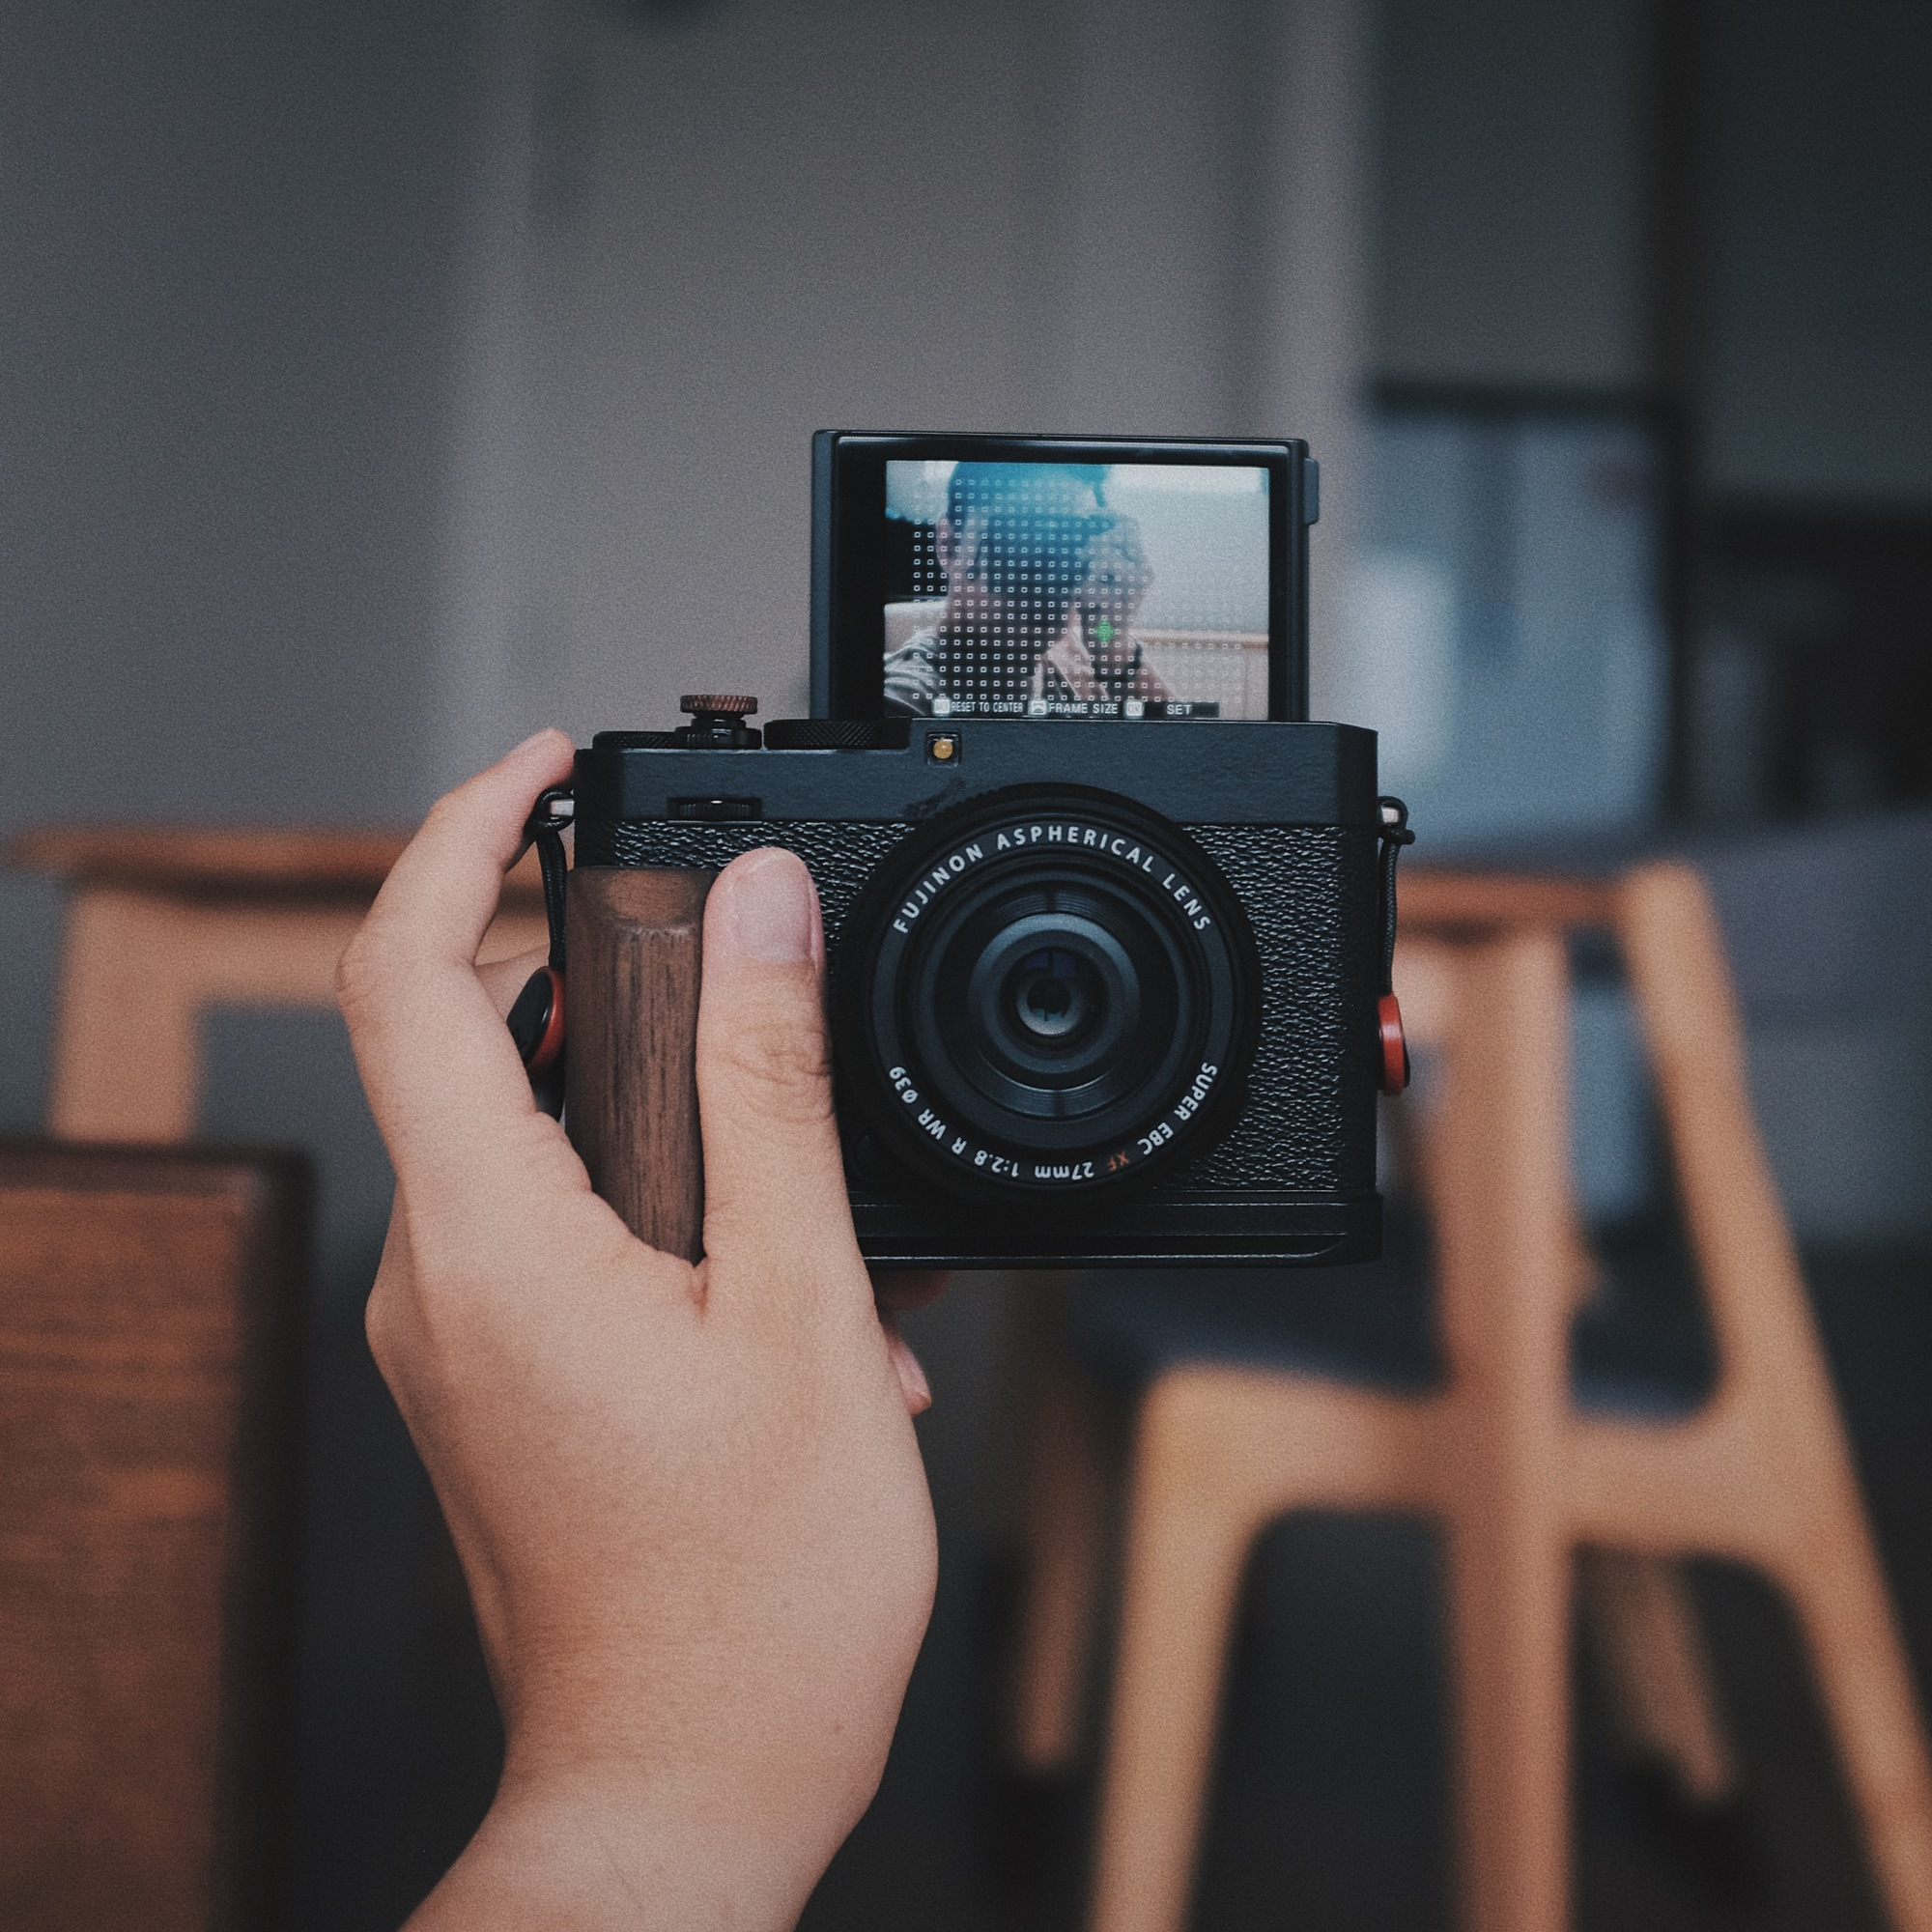
\includegraphics[width=\linewidth]{\envfinaldir/coverpic-prod.jpg}\par
            % \vskip 30pt
            \vfill

            \normalsize\rmfamily\scshape
            \copyright{} The Web Digest Project \hfill\large \envdatestr
        \end{center}
    \end{titlepage}
    % \restoregeometry
}
\newcommand{\simplehref}[1]{%
    \textcolor{blue!80!green}{\href{#1}{#1}}%
}
\renewcommand{\contentsname}{\center\Huge\sffamily\bfseries Contents\par\vskip 20pt}
\newcounter{ipartcounter}
\setcounter{ipartcounter}{0}
\newcommand{\ipart}[1]{
    % \vskip 20pt
    \clearpage
    \stepcounter{ipartcounter}
    \phantomsection
    \addcontentsline{toc}{chapter}{#1}
    % \begin{center}
    %     \Huge
    %     \sffamily\bfseries
    %     #1
    % \end{center}
    % \vskip 20pt plus 7pt
}
\newcounter{ichaptercounter}
\setcounter{ichaptercounter}{0}
\newcommand{\ichapter}[1]{
    % \vskip 20pt
    \clearpage
    \stepcounter{ichaptercounter}
    \phantomsection
    \addcontentsline{toc}{section}{\numberline{\arabic{ichaptercounter}}#1}
    \begin{center}
        \Huge
        \sffamily\bfseries
        #1
    \end{center}
    \vskip 20pt plus 7pt
}
\newcommand{\entrytitlefont}[1]{\subsection*{\raggedright\Large\sffamily\bfseries#1}}
\newcommand{\entryitemGeneric}[2]{
    % argv: title, url
    \parbox{\linewidth}{
        \entrytitlefont{#1}\par\vskip 5pt
        \footnotesize\ttfamily\mdseries
        \simplehref{#2}
    }\vskip 11pt plus 11pt minus 1pt
}
\newcommand{\entryitemGithub}[3]{
    % argv: title, url, desc
    \parbox{\linewidth}{
        \entrytitlefont{#1}\par\vskip 5pt
        \footnotesize\ttfamily\mdseries
        \simplehref{#2}\par\vskip 5pt
        \small\rmfamily\mdseries#3
    }\vskip 11pt plus 11pt minus 1pt
}
\newcommand{\entryitemAp}[3]{
    % argv: title, url, desc
    \parbox{\linewidth}{
        \entrytitlefont{#1}\par\vskip 5pt
        \footnotesize\ttfamily\mdseries
        \simplehref{#2}\par\vskip 5pt
        \small\rmfamily\mdseries#3
    }\vskip 11pt plus 11pt minus 1pt
}
\newcommand{\entryitemHackernews}[3]{
    % argv: title, hnurl, rawurl
    % \parbox{\linewidth}{
    %     \entrytitlefont{#1}\par\vskip 5pt
    %     \footnotesize\ttfamily\mdseries
    %     \simplehref{#3}\par
    %     \textcolor{black!50}{\href{#2}{#2}}
    % }\vskip 11pt plus 11pt minus 1pt
    \begin{minipage}{\linewidth}
            \entrytitlefont{#1}\par\vskip 5pt
            \footnotesize\ttfamily\mdseries
            \simplehref{#3}\par
            \textcolor{black!50}{\href{#2}{#2}}
    \end{minipage}\par\vskip 11pt plus 11pt minus 1pt
}







\begin{document}

\makeheader

\tableofcontents\clearpage




\ipart{Developers}
\ichapter{Hacker News}
\entryitemTwoLinks{Jeff Bezos' revamp of 'Washington Post' opinions leads editor to quit}{https://news.ycombinator.com/item?id=43188749}{https://www.npr.org/2025/02/26/nx-s1-5309725/jeff-bezos-washington-post-opinion-section}

\entryitemTwoLinks{Replace OCR with Vision Language Models}{https://news.ycombinator.com/item?id=43187209}{https://github.com/vlm-run/vlmrun-cookbook/blob/main/notebooks/01\_schema\_showcase.ipynb}

\entryitemTwoLinks{Cross Views}{https://news.ycombinator.com/item?id=43186413}{https://moultano.wordpress.com/2025/02/24/you-should-make-cross-views/}

\entryitemTwoLinks{Show HN: I got laid off from Meta and created a minor hit on Steam}{https://news.ycombinator.com/item?id=43186406}{https://news.ycombinator.com/item?id=43186406}

\entryitemTwoLinks{The man who spent forty-two years at the Beverly Hills Hotel pool (1993)}{https://news.ycombinator.com/item?id=43186050}{https://www.newyorker.com/magazine/1993/02/22/beverly-hills-hotel-paradise-lost}

\entryitemTwoLinks{DARPA Large Bio-Mechanical Space Structures}{https://news.ycombinator.com/item?id=43185769}{https://sam.gov/opp/49c9fac62ef249f19cda8b436a095d3b/view}

\entryitemTwoLinks{Alexa+}{https://news.ycombinator.com/item?id=43185446}{https://www.aboutamazon.com/news/devices/new-alexa-generative-artificial-intelligence}

\entryitemTwoLinks{Launch HN: Maritime Fusion (YC W25) – Fusion Reactors for Ships}{https://news.ycombinator.com/item?id=43185246}{https://news.ycombinator.com/item?id=43185246}

\entryitemTwoLinks{Slack Is Down}{https://news.ycombinator.com/item?id=43184878}{https://slack-status.com/2025-02/1b757d1d0f444c34}

\entryitemTwoLinks{Jeff Bezos exerts more control of Washington Post opinion}{https://news.ycombinator.com/item?id=43184762}{https://deadline.com/2025/02/jeff-bezos-washington-post-opinion-1236302292/}

\entryitemTwoLinks{ForeverVM: Run AI-generated code in stateful sandboxes that run forever}{https://news.ycombinator.com/item?id=43184686}{https://forevervm.com/}

\entryitemTwoLinks{TypeScript types can run DOOM [video]}{https://news.ycombinator.com/item?id=43184291}{https://www.youtube.com/watch?v=0mCsluv5FXA}

\entryitemTwoLinks{Show HN: A Database Written in Golang}{https://news.ycombinator.com/item?id=43183891}{https://github.com/Sahilb315/AtomixDB}

\entryitemTwoLinks{Show HN: Breakout with a roguelite/vampire survivor twist}{https://news.ycombinator.com/item?id=43183131}{https://breakout.lecaro.me/}

\entryitemTwoLinks{State of emergency declared after blackout plunges most of Chile into darkness}{https://news.ycombinator.com/item?id=43182892}{https://www.cnn.com/2025/02/25/americas/chile-blackout-14-regions-intl-latam/index.html}

\entryitemTwoLinks{The Miserable State of Modems and Mobile Network Operators}{https://news.ycombinator.com/item?id=43182854}{https://blog.golioth.io/the-miserable-state-of-modems-and-mobile-network-operators/}

\entryitemTwoLinks{Automattic Hit with Class Action over WP Engine Dispute}{https://news.ycombinator.com/item?id=43182576}{https://www.therepository.email/automattic-hit-with-class-action-over-wp-engine-dispute-accused-of-anti-competitive-tactics}

\entryitemTwoLinks{The FFT Strikes Back: An Efficient Alternative to Self-Attention}{https://news.ycombinator.com/item?id=43182325}{https://arxiv.org/abs/2502.18394}

\entryitemTwoLinks{Show HN: Telescope – an open-source web-based log viewer for logs in ClickHouse}{https://news.ycombinator.com/item?id=43181862}{https://github.com/iamtelescope/telescope}

\entryitemTwoLinks{Iterated Log Coding}{https://news.ycombinator.com/item?id=43181610}{https://adamscherlis.github.io/blog/iterlog-coding/}\ichapter{Phoronix}
\entryitemGeneric{\hskip 0pt{}Git 2.49-rc0 Released With "git backfill", zlib-ng Preparations \& Rust Interface}{https://www.phoronix.com/news/Git-2.49-rc0-Released}

\entryitemGeneric{\hskip 0pt{}AMD EPYC Turin Power Profile Selection Impact On Performance \& Efficiency}{https://www.phoronix.com/review/amd-power-profile-linux}

\entryitemGeneric{\hskip 0pt{}AMD Driver Lands DCC For Multi-Plane Formats With RDNA4, Tiling For Video Buffers}{https://www.phoronix.com/news/Mesa-25.1-Multi-Plane-DCC-RDNA4}

\entryitemGeneric{\hskip 0pt{}Intel Graphics Driver With Linux 6.15 To Allow Tuning The GuC Power Profile}{https://www.phoronix.com/news/Intel-sysfs-GuC-SLPC-Profile}

\entryitemGeneric{\hskip 0pt{}FineIBT-BHI Looks To Be Ready Ahead Of Linux 6.15 To Provide Tougher Kernel Defenses}{https://www.phoronix.com/news/Linux-FineIBT-BHI-TIP}

\entryitemGeneric{\hskip 0pt{}Mesa's Vulkan WSI Now Supports Wayland Color Management}{https://www.phoronix.com/news/Mesa-Vulkan-WSI-HDR-CM}

\entryitemGeneric{\hskip 0pt{}Spectre Mitigations Being Worked On For BPF Programs}{https://www.phoronix.com/news/Speculation-Barriers-BPF}

\entryitemGeneric{\hskip 0pt{}Framework Announces Ryzen AI Max Powered Desktop, Framework Laptop 12}{https://www.phoronix.com/news/Framework-2nd-Gen-Announcements}

\entryitemGeneric{\hskip 0pt{}Christoph Hellwig Steps Down From One Of His Kernel Roles Following Rust Drama}{https://www.phoronix.com/news/Hellwig-DMA-Helpers-Removed}\ichapter{Dribbble}
\entryitemGeneric{\hskip 0pt{}Ramotion Logo Design}{https://dribbble.com/shots/25582478-Ramotion-Logo-Design}

\entryitemGeneric{\hskip 0pt{}Letter a}{https://dribbble.com/shots/25680095-Letter-a}

\entryitemGeneric{\hskip 0pt{}auren - logo design}{https://dribbble.com/shots/25681046-auren-logo-design}

\entryitemGeneric{\hskip 0pt{}Block13 Skateboards \& Sreetwear}{https://dribbble.com/shots/25683504-Block13-Skateboards-Sreetwear}

\entryitemGeneric{\hskip 0pt{}Quokka Mascot}{https://dribbble.com/shots/25681470-Quokka-Mascot}

\entryitemGeneric{\hskip 0pt{}Cardi C}{https://dribbble.com/shots/25678066-Cardi-C}

\entryitemGeneric{\hskip 0pt{}R}{https://dribbble.com/shots/25673587-R}

\entryitemGeneric{\hskip 0pt{}Fitme home landing page}{https://dribbble.com/shots/25674639-Fitme-home-landing-page}

\entryitemGeneric{\hskip 0pt{}Triceratops Dino}{https://dribbble.com/shots/25676249-Triceratops-Dino}

\entryitemGeneric{\hskip 0pt{}Illustrated Icons - American Home Shield}{https://dribbble.com/shots/25666386-Illustrated-Icons-American-Home-Shield}

\entryitemGeneric{\hskip 0pt{}Unused Geometric Fox}{https://dribbble.com/shots/25677006-Unused-Geometric-Fox}

\entryitemGeneric{\hskip 0pt{}Tiger Style}{https://dribbble.com/shots/25676567-Tiger-Style}

\entryitemGeneric{\hskip 0pt{}Logo Tip 002. Rhythm in Logo Design}{https://dribbble.com/shots/25674872-Logo-Tip-002-Rhythm-in-Logo-Design}

\entryitemGeneric{\hskip 0pt{}The Business}{https://dribbble.com/shots/25676385-The-Business}

\entryitemGeneric{\hskip 0pt{}Cute Dinosaur}{https://dribbble.com/shots/25671549-Cute-Dinosaur}

\entryitemGeneric{\hskip 0pt{}BNPL service}{https://dribbble.com/shots/25664920-BNPL-service}

\entryitemGeneric{\hskip 0pt{}Wolf Creek Golf Club}{https://dribbble.com/shots/25664483-Wolf-Creek-Golf-Club}

\entryitemGeneric{\hskip 0pt{}Business illustration set}{https://dribbble.com/shots/25661493-Business-illustration-set}

\entryitemGeneric{\hskip 0pt{}b}{https://dribbble.com/shots/25663031-b}

\entryitemGeneric{\hskip 0pt{}ProAWS Logo Design}{https://dribbble.com/shots/25661915-ProAWS-Logo-Design}

\entryitemGeneric{\hskip 0pt{}—From Archive (Pt. 8)}{https://dribbble.com/shots/25663911--From-Archive-Pt-8}

\entryitemGeneric{\hskip 0pt{}Form Golf ID}{https://dribbble.com/shots/25660910-Form-Golf-ID}

\entryitemGeneric{\hskip 0pt{}Shooting Ladybug - Make a wish! Nagare Mushi}{https://dribbble.com/shots/25659882-Shooting-Ladybug-Make-a-wish-Nagare-Mushi}

\entryitemGeneric{\hskip 0pt{}Crypto Wallet App Design}{https://dribbble.com/shots/25657576-Crypto-Wallet-App-Design}


\ipart{Developers~~~~(zh-Hans)}
\ichapter{Solidot}
\entryitemGeneric{\hskip 0pt{}Y 孵化器支持的 AI 公司被批评其产品是在虐待工厂工人}{https://www.solidot.org/story?sid=80658}

\entryitemGeneric{\hskip 0pt{}前工业化社群睡眠时间更短}{https://www.solidot.org/story?sid=80657}

\entryitemGeneric{\hskip 0pt{}高通和 Google 合作为 Android 提供最高八年的更新}{https://www.solidot.org/story?sid=80656}

\entryitemGeneric{\hskip 0pt{}皮尤调查发现大部分美国工人避用 AI 聊天机器人}{https://www.solidot.org/story?sid=80655}

\entryitemGeneric{\hskip 0pt{}Mozilla 重申会继续支持 Manifest v2 扩展}{https://www.solidot.org/story?sid=80654}

\entryitemGeneric{\hskip 0pt{}Framework 推出三款新产品,包括 128GB 内存 Ryzen AI Max+ 395 小主机}{https://www.solidot.org/story?sid=80653}

\entryitemGeneric{\hskip 0pt{}Google 发布免费版编程助手 Gemini Code Assist}{https://www.solidot.org/story?sid=80652}

\entryitemGeneric{\hskip 0pt{}丹麦将禁止初中小学生在学校以及课外俱乐部使用手机}{https://www.solidot.org/story?sid=80651}

\entryitemGeneric{\hskip 0pt{}Christoph Hellwig 不再担任 DMA 维护者}{https://www.solidot.org/story?sid=80650}

\entryitemGeneric{\hskip 0pt{}火星上的古代海滩显示它曾经有海洋}{https://www.solidot.org/story?sid=80649}

\entryitemGeneric{\hskip 0pt{}未知疾病在刚果杀死了逾 50 人}{https://www.solidot.org/story?sid=80648}

\entryitemGeneric{\hskip 0pt{}短期摄入大量高热量饮食会改变大脑模式}{https://www.solidot.org/story?sid=80647}

\entryitemGeneric{\hskip 0pt{}特斯拉汽车欧洲 1 月销量暴跌 45\%}{https://www.solidot.org/story?sid=80645}

\entryitemGeneric{\hskip 0pt{}Aqualung 2.0 释出}{https://www.solidot.org/story?sid=80644}

\entryitemGeneric{\hskip 0pt{}微软将第 11 代前的英特尔处理器移出 Windows 11 24H2 兼容列表 }{https://www.solidot.org/story?sid=80643}

\entryitemGeneric{\hskip 0pt{}朝鲜黑客如何盗走 15 亿美元加密货币}{https://www.solidot.org/story?sid=80642}

\entryitemGeneric{\hskip 0pt{}Gmail 用 QR 码取代短信验证}{https://www.solidot.org/story?sid=80641}

\entryitemGeneric{\hskip 0pt{}2024 年大气二氧化碳浓度增幅创新高}{https://www.solidot.org/story?sid=80640}

\entryitemGeneric{\hskip 0pt{}中国主要电视机品牌出货量首超韩国}{https://www.solidot.org/story?sid=80639}

\entryitemGeneric{\hskip 0pt{}微软推出广告版 Microsoft Office}{https://www.solidot.org/story?sid=80638}\ichapter{V2EX}
\entryitemGeneric{\hskip 0pt{}[问与答] 一般国外的云服务器除了亚马逊和 google 这些大厂商,还可以去哪里买云服务器,靠谱点的,有大佬推荐的吗?}{https://www.v2ex.com/t/1114487}

\entryitemGeneric{\hskip 0pt{}[职场话题] 摸鱼时间!聊聊所谓的``熟练''和``精通''}{https://www.v2ex.com/t/1114486}

\entryitemGeneric{\hskip 0pt{}[程序员] 有一段时间没来了,说说我不上班后最新的收入情况}{https://www.v2ex.com/t/1114485}

\entryitemGeneric{\hskip 0pt{}[问与答] 淘宝某商家客服要求提供真实姓名信息以供快递实名是否有猫腻}{https://www.v2ex.com/t/1114484}

\entryitemGeneric{\hskip 0pt{}[问与答] 海淘什么东西有点价值啊? 人肉带货,可惜本身低消费,不知道富豪圈的消费方式,请分享。 🤜🤛}{https://www.v2ex.com/t/1114483}

\entryitemGeneric{\hskip 0pt{}[酷工作] 腾讯文档团队前端开发暑期实习生招聘}{https://www.v2ex.com/t/1114482}

\entryitemGeneric{\hskip 0pt{}[职场话题] AI 发展的整体方向对于程序员是削弱还是加强?}{https://www.v2ex.com/t/1114481}

\entryitemGeneric{\hskip 0pt{}[问与答] 欠款人抵给我两套音响,如何止损?}{https://www.v2ex.com/t/1114480}

\entryitemGeneric{\hskip 0pt{}[分享创造] 有一段时间没来了,说说我最新的项目进展}{https://www.v2ex.com/t/1114479}

\entryitemGeneric{\hskip 0pt{}[程序员] [有偿求助] Mac 系统 USB 驱动开发,搞定直接>888 RMB<红包}{https://www.v2ex.com/t/1114478}

\entryitemGeneric{\hskip 0pt{}[分享创造] 开源个小工具——多语言翻译生成}{https://www.v2ex.com/t/1114477}

\entryitemGeneric{\hskip 0pt{}[分享发现] 小米有品发布「口袋玲珑 全尺寸折叠键盘多功能主机」}{https://www.v2ex.com/t/1114475}

\entryitemGeneric{\hskip 0pt{}[问与答] 两台手机的必要性?为什么我参加的商务活动,大佬几乎都是一台手机?}{https://www.v2ex.com/t/1114473}

\entryitemGeneric{\hskip 0pt{}[程序员] win7 重装系统,在展开 Windows 文件时卡死,怎么解决}{https://www.v2ex.com/t/1114472}

\entryitemGeneric{\hskip 0pt{}[酷工作] 校招内推 | 拼多多 PDD | 简历优先安排}{https://www.v2ex.com/t/1114471}

\entryitemGeneric{\hskip 0pt{}[分享发现] warp.dev windows 可以下载了}{https://www.v2ex.com/t/1114470}

\entryitemGeneric{\hskip 0pt{}[上海] 请教上海这边哪些公司有测开岗位,压力小一些}{https://www.v2ex.com/t/1114469}

\entryitemGeneric{\hskip 0pt{}[分享创造] 我也开源一款 markdown 所见即所得编辑器,支持 slash commands,支持 npm 安装}{https://www.v2ex.com/t/1114468}

\entryitemGeneric{\hskip 0pt{}[问与答] 哪些海外品牌手机支持双卡双待+双 VX+双 QQ 呢?}{https://www.v2ex.com/t/1114467}

\entryitemGeneric{\hskip 0pt{}[生活] 今日思辨之交警执法的问题}{https://www.v2ex.com/t/1114465}

\entryitemGeneric{\hskip 0pt{}[程序员] 请教一个 nginx+ PHP 本地搭建 wordpress,使用 frp 内网穿透,并通过 nginx 反向代理问题?}{https://www.v2ex.com/t/1114464}

\entryitemGeneric{\hskip 0pt{}[投资] 富途定投纳斯达克 QQQ 一定要用美元吗}{https://www.v2ex.com/t/1114462}

\entryitemGeneric{\hskip 0pt{}[程序员] App Store 上架求助,公安备案流程疑惑}{https://www.v2ex.com/t/1114460}

\entryitemGeneric{\hskip 0pt{}[酷工作] [北京] AI 应用层初创团队招募 全栈开发工程师(移动端+后端)}{https://www.v2ex.com/t/1114459}

\entryitemGeneric{\hskip 0pt{}[分享创造] [送码] 挥拍吧 app,你的专业羽毛球运动分析助手, UI 全新升级}{https://www.v2ex.com/t/1114458}

\entryitemGeneric{\hskip 0pt{}[问与答] shell 一键脚本的执行命令可以被导出吗?}{https://www.v2ex.com/t/1114457}

\entryitemGeneric{\hskip 0pt{}[程序员] 独立开发者的标杆: Pieter Levels}{https://www.v2ex.com/t/1114456}

\entryitemGeneric{\hskip 0pt{}[互联网] 互联网失去了讨论的空间}{https://www.v2ex.com/t/1114455}

\entryitemGeneric{\hskip 0pt{}[macOS] 如何使用 iPhone 当 Mac 摄像头实现 60fps 视频录制的方案}{https://www.v2ex.com/t/1114454}

\entryitemGeneric{\hskip 0pt{}[问与答] 努比亚手机内嵌全尺寸 deepseek,这个是怎么做到的?}{https://www.v2ex.com/t/1114452}

\entryitemGeneric{\hskip 0pt{}[数据库] TiDB 的 sql 查询为什么这么慢呀,是我打开的方式不对吗?}{https://www.v2ex.com/t/1114450}

\entryitemGeneric{\hskip 0pt{}[香港] MasterCard 内地 10\% 返现退款问题}{https://www.v2ex.com/t/1114449}

\entryitemGeneric{\hskip 0pt{}[生活] 盛年不重来,及时当勉励}{https://www.v2ex.com/t/1114448}

\entryitemGeneric{\hskip 0pt{}[宽带症候群] 是否该取消掉宽带}{https://www.v2ex.com/t/1114447}

\entryitemGeneric{\hskip 0pt{}[iOS] LiveCommunicationKit 在外版设备可以自动 fallback 成 CallKit?}{https://www.v2ex.com/t/1114446}

\entryitemGeneric{\hskip 0pt{}[Linux] Linux 使用 systemd 作为软路由,以及 IPV6 DHCPv6-PD}{https://www.v2ex.com/t/1114445}

\entryitemGeneric{\hskip 0pt{}[职场话题] V 站有字节 Flow AI 团队的同学吗?}{https://www.v2ex.com/t/1114444}

\entryitemGeneric{\hskip 0pt{}[程序员] Rustdesk 用户登录问题}{https://www.v2ex.com/t/1114443}

\entryitemGeneric{\hskip 0pt{}[宽带症候群] 有一奇怪的网络超时问题}{https://www.v2ex.com/t/1114442}

\entryitemGeneric{\hskip 0pt{}[分享发现] 字节对标 cursor 的 IDE, trae 还不错}{https://www.v2ex.com/t/1114441}

\entryitemGeneric{\hskip 0pt{}[分享创造] 用 Cursor 写个赛车游戏玩下}{https://www.v2ex.com/t/1114440}

\entryitemGeneric{\hskip 0pt{}[宽带症候群] 湖南电信获取不到 IPV6 了}{https://www.v2ex.com/t/1114439}

\entryitemGeneric{\hskip 0pt{}[创业组队] 🚀 [招募技术合伙人] AI+社交 | 寻找全栈 / AI 工程师,共建社交新模式}{https://www.v2ex.com/t/1114437}

\entryitemGeneric{\hskip 0pt{}[云计算] nextjs 项目,想要优化国内访问速度,应该部署到阿里云还是腾讯云。}{https://www.v2ex.com/t/1114436}

\entryitemGeneric{\hskip 0pt{}[微信] iPhone 云测试微信小程序 有什么好推荐?}{https://www.v2ex.com/t/1114434}

\entryitemGeneric{\hskip 0pt{}[OpenAI] deepseek 刚放开充值就降价}{https://www.v2ex.com/t/1114433}

\entryitemGeneric{\hskip 0pt{}[职场话题] 年初裁员,想要抱团取暖}{https://www.v2ex.com/t/1114432}

\entryitemGeneric{\hskip 0pt{}[微信] 为什么微信不推出聊天记录云存储功能?付费也行。}{https://www.v2ex.com/t/1114431}

\entryitemGeneric{\hskip 0pt{}[职场话题] offer 方向二选一 求 v 友们指点迷津}{https://www.v2ex.com/t/1114430}

\entryitemGeneric{\hskip 0pt{}[OpenAI] ChatGPT 的 deep research 开启后,使用的模型和你目前模型选择器的模型有关系吗}{https://www.v2ex.com/t/1114429}


\ipart{Generic News}
\ichapter{AP News}
\entryitemWithDescription{\hskip 0pt{}Thieves nab pricey bulldogs from a Colorado pet store after faking a seizure, sheriff says}{https://apnews.com/article/92cb0d90418fc204e5ba72150b5fd293}{}

\entryitemWithDescription{\hskip 0pt{}A whale caught in fishing nets has been freed off Poland's Baltic coast}{https://apnews.com/article/8beaa130246b3c570fc5b491c6e5a09f}{}

\entryitemWithDescription{\hskip 0pt{}Amazon's new AI-powered Alexa promises to be your `best friend in a digital world' for a monthly fee}{https://apnews.com/article/017c17bddfa6742d1e78873cdda3663f}{}

\entryitemWithDescription{\hskip 0pt{}Apple will fix iPhone glitch that suggests replacing the word `racist' with `Trump'}{https://apnews.com/article/d80f88d69f6ceac585904f2faa2a9212}{}

\entryitemWithDescription{\hskip 0pt{}Southwest Airlines flight abruptly rises to avoid another plane crossing Chicago runway}{https://apnews.com/article/e0abb86c91ea54a751cc917ae97d2d11}{}

\entryitemWithDescription{\hskip 0pt{}Diana Taurasi of the Phoenix Mercury retires after 20 WNBA seasons, 3 titles and 6 Olympic golds}{https://apnews.com/article/cacc627783d5a6b418425d610ac58b86}{}

\entryitemWithDescription{\hskip 0pt{}Slack platform down as users report service outage}{https://apnews.com/article/1d010c3ae302c7d4831a827273b45b81}{}

\entryitemWithDescription{\hskip 0pt{}Michigan veterinarian faces theft charge after refusing to return homeless man's dog}{https://apnews.com/article/fc66ca92499cc3bc90faf7abb3e7f2d0}{}

\entryitemWithDescription{\hskip 0pt{}SWAT team raided the wrong Denver apartment and traumatized two young girls, lawsuit says}{https://apnews.com/article/f765f56658aaac40302d8d276f61112b}{}

\entryitemWithDescription{\hskip 0pt{}Losing a pet can cut deeper than many people realize. Here's how friends can help}{https://apnews.com/article/a63d5b3a3fd3b8d303aca3cec50c032c}{}

\entryitemWithDescription{\hskip 0pt{}Luxury home at risk of tumbling into Cape Cod Bay over removal dispute is demolished}{https://apnews.com/article/bf3f32883558b7d91bdb318ce3f68ecd}{}

\entryitemWithDescription{\hskip 0pt{}Woman injured on Harry Potter theme park ride in California is awarded \$7.25 million}{https://apnews.com/article/f34b01602082534f633b49147966ff1a}{}

\entryitemWithDescription{\hskip 0pt{}Ravens GM calls sexual misconduct allegations against Justin Tucker `concerning'}{https://apnews.com/article/f2109f3ddcd6ac8be8edde879912cf31}{}






\clearpage
\leavevmode\vfill
\footnotesize

Copyright \copyright{} 2023-2025 Neruthes and other contributors.

This document is published with CC BY-NC-ND 4.0 license.

The entries listed in this newsletter may be copyrighted by their respective creators.

This newsletter is generated by the Web Digest project.

The newsletters are also delivered via Telegram channel \CJKunderline{\href{https://t.me/webdigestchannel}{https://t.me/webdigestchannel}}.\\
RSS feed is available at \CJKunderline{\href{https://webdigest.pages.dev/rss.xml}{https://webdigest.pages.dev/rss.xml}}.

This newsletter is available in PDF at
\CJKunderline{\href{https://webdigest.pages.dev/}{https://webdigest.pages.dev/}}.

The source code being used to generate this newsletter is available at\\
\CJKunderline{\href{https://github.com/neruthes/webdigest}{https://github.com/neruthes/webdigest}}.

This newsletter is also available in
\CJKunderline{\href{http://webdigest.pages.dev/readhtml/\envyear/WebDigest-20250227.html}{HTML}} and
\CJKunderline{\href{https://github.com/neruthes/webdigest/blob/master/markdown/\envyear/WebDigest-20250227.md}{Markdown}}.


\coverpic{}{}


\end{document}
